\ifdefined\isfinal\documentclass[final]{dune}\else\documentclass{dune}\fi
\pdfoutput=1            % must be in first 5 lines so arXiv finds it

% Edit: set this line to match this volume's sub-directories holding figures
\graphicspath{ {figures/}{guidance/figures/}{guidance/generated/} }

% Leave as is.
% This includes all common settings which are related to this
% particular CDR's set of volumes.
% This file is to hold any special settings for a particular CDR
% Things that are generic to CDRs in general go in cdr.cls.
% Probably no \usepackages should be here.

%\usepackage[pdftex,pdfpagelabels,bookmarks]{hyperref}



% This holds definitions of macros to enforce consistency in names.

% This file is the sole location for such definitions.  Check here to
% learn what there is and add new ones only here.  

% also see units.tex for units.

%%% Common terms

% Check here first, don't reinvent existing ones, add any novel ones.
% Use \xspace.

\def\expshort{LBN\xspace}
\def\explong{The Neutrino Experiment\xspace}
\def\thevolumenumber{0}


% Things about oscillation
%
\newcommand{\numu}{$\nu_\mu$\xspace}
\newcommand{\nue}{$\nu_e$\xspace}
\newcommand{\nutau}{$\nu_\tau$\xspace}

\newcommand{\anumu}{$\bar\nu_\mu$\xspace}
\newcommand{\anue}{$\bar\nu_e$\xspace}
\newcommand{\anutau}{$\bar\nu_\tau$\xspace}

\newcommand{\dm}[1]{$\Delta m^2_{#1}$\xspace} % example: \dm{12}

\newcommand{\sinst}[1]{$\sin^2\theta_{#1}$\xspace} % example \sinst{12}
\newcommand{\sinstt}[1]{$\sin^22\theta_{#1}$\xspace}  % example \sinstt{12}

\newcommand{\deltacp}{$\delta_{\rm CP}$\xspace}   % example \deltacp
\newcommand{\mdeltacp}{$\delta_{\rm CP}$}   %%%%%%%%%%  <--- missing something; what's the m for?

\newcommand{\nuxtonux}[2]{$\nu_{#1} \to \nu_{#2}$\xspace}  % example \nuxtonux23 (no {...} )
\newcommand{\numutonumu}{\nuxtonux{\mu}{\mu}}
\newcommand{\numutonue}{\nuxtonux{\mu}{e}}
% Add chi sqd MH?  avg delta chi sqd?

% atmospheric neutrinos and PDK
\newcommand{\ptoknubar}{$p^+ \rightarrow K^+ \overline{\nu}$\xspace}
\newcommand{\ptoepizero}{$p^+ \rightarrow e^+ \pi^0$\xspace}

% Names of expts or detectors
\newcommand{\cherenkov}{Cherenkov\xspace}
\newcommand{\kamland}{KamLAND\xspace}
\newcommand{\kkande}{Kamiokande\xspace}  %%%% <---- changed to make shorter
\newcommand{\superk}{Super--Kamiokande\xspace}
\newcommand{\hyperk}{Hyper--Kamiokande\xspace}
\newcommand{\miniboone}{MiniBooNE\xspace}
\newcommand{\minerva}{MINER$\nu$A\xspace}
\newcommand{\nova}{NO$\nu$A\xspace}
\newcommand{\numi}{NuMI\xspace}
\newcommand{\lariat}{LArIAT\xspace}
\newcommand{\argoneut}{ArgoNeuT\xspace}

% Random
\newcommand{\lartpc}{LArTPC\xspace}
\newcommand{\SURF}{Sanford Underground Research Facility\xspace}
\newcommand{\globes}{GLoBES\xspace}
\newcommand{\larsoft}{LArSoft\xspace}
\newcommand{\snowglobes}{SNOwGLoBES\xspace}

% Isotopes
\def\argon40{$^{40}$Ar}  %%%%%       <--- \Ar40 doesn't work; don't know why
\def\Ar39{$^{39}$Ar}
\def\Cl40{$^{40}$Cl}
\def\K40{$^{40}$K}
\def\B8{$^{8}$B}

% Parameters
\def\driftvelocity{\SI{1.6}{\milli\meter/\micro\second}\xspace}
\def\lartemp{\SI{88}\,K\xspace}
% What other parameters to include?  Wire spacings? Drift lengths? Decay pipe length?

% This holds definitions of macros to enforce consistency in units.

% This file is the sole location for such definitions.  Check here to
% learn what there is and add new ones only here.  

% also see defs.tex for names.


% see
%  http://ctan.org/pkg/siunitx
%  http://mirrors.ctan.org/macros/latex/contrib/siunitx/siunitx.pdf

% Examples:
%  % angles
%  \ang{1.5} off-axis
%
%  % just a unit
%  \si{\kilo\tonne}
%
%  % with a value:
%  \SI{10}{\mega\electronvolt}

%  range of values:
% \SIrange{60}{120}{\GeV}

% some shorthand notation
%\DeclareSIUnit \MBq {\mega\Bq}
\DeclareSIUnit \s {\second}
\DeclareSIUnit \MB {\mega\byte}
\DeclareSIUnit \GB {\giga\byte}
\DeclareSIUnit \TB {\tera\byte}
\DeclareSIUnit \PB {\peta\byte}
\DeclareSIUnit \Mbps {\mega\bit/\s}
\DeclareSIUnit \Gbps {\giga\bit/\s}
\DeclareSIUnit \Tbps {\tera\bit/\s}
\DeclareSIUnit \Pbps {\peta\bit/\s}
\DeclareSIUnit \kton {\kilo\tonne} % changed  back to kton
\DeclareSIUnit \kt {\kilo\tonne}
\DeclareSIUnit \Mt {\mega\tonne}
\DeclareSIUnit \eV {\electronvolt}
\DeclareSIUnit \keV {\kilo\electronvolt}
\DeclareSIUnit \MeV {\mega\electronvolt}
\DeclareSIUnit \GeV {\giga\electronvolt}
\DeclareSIUnit \m {\meter}
\DeclareSIUnit \cm {\centi\meter}
\DeclareSIUnit \in {\inchcommand}
\DeclareSIUnit \km {\kilo\meter}
\DeclareSIUnit \kV {\kilo\volt}
\DeclareSIUnit \kW {\kilo\watt}
\DeclareSIUnit \MW {\mega\watt}
\DeclareSIUnit \MHz {\mega\hertz}
\DeclareSIUnit \mrad {\milli\radian}
\DeclareSIUnit \year {year}
\DeclareSIUnit \POT {POT}
\DeclareSIUnit \sig {$\sigma$}
\DeclareSIUnit\parsec{pc}
\DeclareSIUnit\lightyear{ly}
\DeclareSIUnit\foot{ft}
\DeclareSIUnit\ft{ft}
\DeclareSIUnit \ppb{ppb}
\DeclareSIUnit \ppt{ppt}
\DeclareSIUnit \samples{S}

% for a bare kt-year
\def\ktyr{\si[inter-unit-product=\ensuremath{{}\cdot{}}]{\kt\year}\xspace}
\def\Mtyr{\si[inter-unit-product=\ensuremath{{}\cdot{}}]{\Mt\year}\xspace}
\def\msr{\si[inter-unit-product=\ensuremath{{}\cdot{}}]{\meter\steradian}\xspace}
\def\ktMWyr{\si[inter-unit-product=\ensuremath{{}\cdot{}}]{\kt\MW\year}\xspace}

% used for hyphen, obsolete now: \newcommand{\SIadj}[2]{\SI[number-unit-product = -]{#1}{#2}}
% change command definition Nov 2017 in case people copy e.g., \ktadj from CDR text.
% E.g., \ktadj{10} now renders the same as \SI{10}{\kt}
\newcommand{\SIadj}[2]{\SI{#1}{#2}}

% Adjective form of some common units (Nov 2107 changed to be same as normal form, no hyphen)
% "the 10-kt detector"

\newcommand{\ktadj}[1]{\SIadj{#1}{\kt}}
% "the 1,300-km baseline"
\newcommand{\kmadj}[1]{\SIadj{#1}{\km}}
% "a 567-keV endpoint"
\newcommand{\keVadj}[1]{\SIadj{#1}{\keV}}
% "Typical 20-MeV event"
\newcommand{\MeVadj}[1]{\SIadj{#1}{\MeV}}
% "Typical 2-GeV event"
\newcommand{\GeVadj}[1]{\SIadj{#1}{\GeV}}
% "the 1.2-MW beam"
\newcommand{\MWadj}[1]{\SIadj{#1}{\MW}}
% "the 700-kW beam"
\newcommand{\kWadj}[1]{\SIadj{#1}{\kW}}
% "the 100-tonne beam"
\newcommand{\tonneadj}[1]{\SIadj{#1}{\tonne}}
% "the 4,850-foot depth beam"
\newcommand{\ftadj}[1]{\SIadj{#1}{\ft}}
%

% Mass exposure, people like to put dots between the units
% \newcommand{\ktyr}[1]{\SI[inter-unit-product=\ensuremath{{}\cdot{}}]{#1}{\kt\year}}
% must make usage of \ktyr above consistent with this one before turning on

% Beam x mass exposure, people like to put dots between the units
\newcommand{\ktmwyr}[1]{\SI[inter-unit-product=\ensuremath{{}\cdot{}}]{#1}{\kt\MW\year}}



% Set the major title, consistently across all volumes
\renewcommand\thevolumetitle{Technical Design Report \\ \explong}

% Do this here to make use of the experiment name and title macro
\hypersetup{
    pdftitle={\expshort TDR \thevolumesubtitle},
    pdfauthor={\expshort Collaboration},
    final=true,
    colorlinks=false,
    linktocpage=true,
    linkbordercolor=blue,
    citebordercolor=green,
    urlbordercolor=magenta,
    filecolor=black,
    pdfpagemode=UseOutlines,
    pdfborderstyle={/S/U},  
}





% Edit: set main and subtitles
\renewcommand\thevolumetitle{Guidance on Producing \LaTeX{} Documents for DUNE/LBNF}
\renewcommand\thevolumesubtitle{Instructions and Example}

\begin{document}
% Leave as is. Initial content common to all volumes.
% This should be \input first thing after \begin{document}


\pagestyle{empty}

\begin{center}
  {\Huge  \thevolumetitle}

  \vspace{5mm}

  {\LARGE \thevolumesubtitle}

   \vspace{5mm}
   
   Anne Heavey, Fermilab; technical editor, structure, style \\
   Brett Viren, Brookhaven; LaTeX machinery and GitHub repository\\
   David DeMuth, VCSU; LaTeX, images, general\\
   Nora Ransom, KSU; technical and copy editor
   
 \vspace{5mm}

  \today

  \vspace{5mm}

%  \titleextra
\end{center}



\cleardoublepage


%\includepdf[pages={-}]{tdr-authors.pdf}                        <--- add in later
%\input{dune-institutions} Anne removing for collab review 21 May

\cleardoublepage


\renewcommand{\familydefault}{\sfdefault}
\renewcommand{\thepage}{\roman{page}}
\setcounter{page}{0}

\pagestyle{plain} 

%\clearpage

\textsf{\tableofcontents}
%\clearpage


\textsf{\listoffigures}
%\clearpage

\textsf{\listoftables}
%\clearpage

%For acronym list to appear just after TOC, TOF, TOT
%\printnomenclature
%\clearpage

\iffinal\else
\textsf{\listoftodos}
\clearpage
\fi

\renewcommand{\thepage}{\arabic{page}}
\setcounter{page}{1}

\pagestyle{fancy}

% Set how header/footers look
\renewcommand{\chaptermark}[1]{%
\markboth{Chapter \thechapter:\ #1}{}}
\fancyhead{}
\fancyhead[RO,LE]{\textsf{\footnotesize \thechapter--\thepage}}
\fancyhead[LO,RE]{\textsf{\footnotesize \leftmark}}

\fancyfoot{}
\fancyfoot[RO]{\textsf{\footnotesize The DUNE Technical Design Report}}
\fancyfoot[LO]{\textsf{\footnotesize \thedoctitle}}
\fancypagestyle{plain}{}

\renewcommand{\headrule}{\vspace{-4mm}\color[gray]{0.5}{\rule{\headwidth}{0.5pt}}}

% Not all main documents have any citations.
% When not built in "final" mode, add in one citation just to let the
% document build.
% If, after substantial editing a main document still lacks any
% citations then it should have its whole bibliography removed.
%\ifdefined\isfinal\nocite{}\else\nocite{CD0}\fi
\nocite{CD0}


% see also preamble.tex
%\input{common/acronyms}


% Edit: input each chapter file in order

\chapter{General Information}
\label{ch:gen}

This volume gives guidance to authors and editors of DUNE documents such as the CDR, TDRs, and so on. It collects ``wisdom'' learned from 
producing earlier documents, including the DUNE CDR, and we will appreciate 
very much if everyone follows it!  It tries to follows its own guidance so that its \LaTeX{} source
provides an example.  

This has been updated for the DUNE TDR. Earlier versions of this guidance document were updated for other important documents, e.g., the CDR and the ProtoDUNE-SP TDR.  These versions can be found at \url{https://github.com/DUNE/document-guidance/releases/}.


%%%%%%%%%%%%%%%%%%%%%%%%%%%%%%%%%%%%%%%%%%%%%%%%%%%%%%%%%%%%%%%%%%%%
\section{What's on the Document Guidance GitHub Web Page?}
\label{sec:gen-webpage}

Information about using GitHub and building a document is on the web page \url{https://github.com/DUNE/document-guidance}:

\begin{itemize}
\item Four important guidelines about interacting with git that will help avoid headaches!
\item How to get started with GitHub and get the files that you need to edit. See both ``Getting Started'' (at the top) and ``Repository'' further down.  ``Repository'' provides commands to use for interacting with GitHub.
\item How to build the document, in draft format (with extra markup) after you have it downloaded to your local machine.
\item How to build a print-ready document -- even though in principle you don't need to do this, you may want to see how it looks. The technical editors will build the final document.
\item How to access builds of the document run automatically from the content on GitHub.
\item How to get away without authoring in \LaTeX{}...
\end{itemize}

Note about Draft vs. Print format: 

Draft format gives you line numbers, ``fixme'' and other markup notes (see Chapter~\ref{ch:review}), 
faint grey notes (enclosed in a box) near labeled items (headings, figures, tables, etc.) to help you know 
what label was used to reference each particular thing.  
It's easiest to trace things when the labels are meaningful, and for figures, when they match the image filename, so please choose labels carefully. Labels are discussed in Section~\ref{sec:latex-intra-doc-ref}.

%%%%%%%%%%%%%%%%%%%%%%%%%%%%%%%%%%%%%%%%%%%%%%%%%%%%%%%%%%%%%%%%%%%%
\section{What's in the Document Guidance GitHub Repository?}
\label{sec:gen-guidance-repo}

This repository contains code for a document with ``all you need to know'' about using /LBNF/DUNE \LaTeX{}  conventions  -- guidance on syntax, chapter structure, English standards, abbreviations, figures, and other things. Please read through it so that you understand the LBNF/DUNE style and structure for documents.  There is customized \LaTeX{} code that you can copy straight from the source for this document and edit for your content.  This is supposed to make it easy!


%%%%%%%%%%%%%%%%%%%%%%%%%%%%%%%%%%%%%%%%%%%%%%%%%%%%%%%%%%%%%%%%%%%%
\section{What's in the DUNE TDR GitHub Repository?}
\label{sec:gen-repo}

A document maintained in GitHub pertaining to the overall DUNE enterprise, such as the TDR, may consist of multiple \textit{volumes}\footnote{Some volumes may be written in MS Word, external to a GitHub repository.}.  A document repository holds all the files needed to compile each volume of the document (or the document itself, if it's not broken into volumes). This includes both content files and additional files that set up the configuration, 
contain auxiliary text (e.g., acronym lists, citations), or provide definitions or macros (\texttt{defs.tex}), etc.  Most of these other files are maintained by the technical editor and you should not modify them. You may of course add citations, acronyms, and so forth.   More information on these files is given in Chapter~\ref{ch:tech}.

The DUNE TDR repository is set up with a subdirectory for each volume -- this is where you will do the bulk of your work. In the following, \texttt{volname} represents a label for the volume. The content is
arranged as follows:

\begin{description}
\item[\texttt{common}] a top-level directory that houses several configuration-related files and files that are otherwise used by multiple volumes. The ones you are likely to touch are \texttt{defs.tex}, \texttt{tdr-citedb.bib}, and possibly one or another of the acronym files.
\item[\texttt{volname.tex}] the main file (see Section~\ref{sec:tech-mainfile}) for a volume; there will one of these per volume. They are found in the top-level
  directory. They have no significant content themselves; they just use
  ``includes'' to pull together content contained in their component chapter files. Please do NOT modify any volume file!
\item[\texttt{figures/}] top-level subdirectory for any static figures
  shared by more than one volume in the repository. Typically your figures will be volume-specific and you won't add them here.
\item[\texttt{far-detector-(something)-phase/}] The SP and DP Far Detector technologies will have multiple volumes each. Therefore an extra directory level is inserted at the top level for each, to separately collect the SP and the DP sets of volumes.  
\item[\texttt{volname/}] subdirectory holding all content for one particular volume (under directories of previous bullet for detector volumes). You will work within a given volume subdirectory. 
\item[\texttt{volname/chaptername.tex}] holds the content for one chapter of a volume. You will add or edit content in one or more chapter files.
\item[\texttt{volname/figures/}] subdirectory holding any static volume-specific figures. Your figures will usually go here.
\item[\texttt{volname/generated/}] subdirectory holding any generated
  figures (see Section~\ref{sec:graphic-plots} for info on generated files). Your ROOT plots, for example, will go here.
\end{description}

Multi-volume documents will have an established file naming convention (e.g., the
TDR uses ``\texttt{volume-volumename}''.
Specific files hold chapter-level or section-level content and should be named with some
short, descriptive label, e.g., ``\texttt{chapter-chaptername}.''

\hlfix{As of November 2017, the APA volume  of the TDR has its contents structure set. It should serve as a model for structuring other detector element volumes.}{Notice this!}

Please note:
\begin{itemize}
\item Editors may elect to further break up content into per-section files. If so, follow a naming convention such as ``\texttt{chaptername-sectionname.tex}''.
\item Please do not include a volume, chapter, section or figure number in any file name. Their actual numbers will be determined at compile time according to the configuration and the volume's main file. 
\item If you have questions, consult with one of: \\
  Anne Heavey, aheavey@fnal.gov, 630-840-8039 (technical editor)\\
  Brett Viren, bv@bnl.gov or Dave DeMuth, david.demuth@vcsu.edu (help on graphics, \LaTeX{}, git or Overleaf machinery.)
\end{itemize}

%%%%%%%%%%%%%%%%%%%%%%%%%%%%%%%%%%%%%%%%%%%%%%%%%%%%%%%%%%%%%%%%%%%%
\section{Overleaf Editing}
\label{sec:gen-overleaf}

Overleaf is a \LaTeX{} web-based editing utility that provides a real-time WYSIWYG environment. Membership is free: www.overleaf.com

By going into your local git repository an Overleaf importable .zip file is generated via the line command: \texttt{\$ git archive -o latest.zip HEAD}

At Overleaf, select NEW PROJECT
\fixme{instructions not yet complete; also see Technical Proposal page on the dune wiki}

%%%%%%%%%%%%%%%%%%%%%%%%%%%%%%%%%%%%%%%%%%%%%%%%%%%%%%%%%%%%%%%%%%%%
\section{If you read nothing else in this document...}
\label{sec:gen-nothing}

... at least remember that it is here for reference!

%%%%%%%%
\textbf{Macros (Definitions):}

\begin{framed}
We recommend that you use (and add to, as needed) macros defined in \texttt{common/defs.txt} for complicated expressions like 
\begin{verbatim}
$\bar\nu_\mu$.
\end{verbatim}
 Clearly, typing a macro like 
 \begin{verbatim}
\anumu
\end{verbatim} 
is easier and much less error-prone than the full expression.
%\verb|\newcommand{\anumu}{$\bar\nu_\mu$\xspace}|. Clearly, typing \verb|\anumu| is much less error-prone than the full expression.
Find more information in Section~\ref{sec:latex-terms}.
\end{framed}

%%%%%%%%
\textbf{Fixmes:}

\begin{framed}
As in ``fix me!'' If you're not sure about something or you find an error that somebody else has to fix, use:
\begin{verbatim}
\fixme{This is a fixme.}
\end{verbatim}
More info and other options are in Chapter~\ref{ch:review}.
\end{framed}

%%%%%%%%
\textbf{Figures:}

\begin{framed}
\begin{verbatim}
    \begin{dunefigure}[optional caption for LoF]{fig:required-label}
     {required full caption (Credit: xyz)}
    \includegraphics[width=0.8\textwidth]{image-filename}
    \end{dunefigure}
\end{verbatim}
To reference: \verb|See Figure~\ref{fig:required-label}|.
Please make \verb|required-label| the same as \verb|image-filename|. 

Please check that your figures are reasonably sized. We may want to add this document to the arXiv, which has a 10\,MB limit per document; bloated figures can use that up quickly. Find more information in Section~\ref{sec:latex-figures}.
\end{framed}

%%%%%%%%
\textbf{Tables:}

\begin{framed}
\begin{verbatim}
\begin{dunetable}
[The LoT caption]
{cc}
{table-label}
{This is a sample table.}
  Rows & Counts \\ \toprowrule
  Row 1 & First \\ \colhline
  Row 2 & Second \\ \colhline
  Row 3 & Third \\ 
\end{dunetable}
\end{verbatim}
To reference: \verb|See Table~\ref{tab:table-label}|.

Find more information in Section~\ref{sec:latex-tables}.
\end{framed}
%%%%%%%%
\textbf{Citations:}
\begin{framed}
They go in \texttt{common/tdr-citedb.bib}. When adding citations to this file, copy the BibTeX rendering of the citation from \url{http://inspirehep.net} if it exists there. (We have left a well-populated \texttt{common/citedb.bib} in the TDR directory in case you want to search for a citation
 that may have appeared in the CDR, or other DUNE/LBNF document.) E.g.,

\begin{verbatim}
 @article{Gando:2010aa,
      author         = {A.~Gando and others},
      title          = "{Constraints on $\theta_{13}$ from A Three-Flavor ...}",
      journal        = {Phys.Rev.D},
      volume         = {83},
      pages          = {052002},
      year           = {2011},
      note           = {arXiv:1009.4771 [hep-ex]},
}
\end{verbatim}
 To reference it within a file, use, e.g.,  \verb|\cite{Gando:2010aa}|.
Find more information in Section~\ref{sec:latex-cit}.
\end{framed}

%%%%%%%%
\textbf{Sectioning:}

\begin{framed}
\begin{verbatim}
\chapter{A Chapter}
\label{ch:blah}

%%%%%%%%%%%%%%%%%%%%%%%%%%%%%%%%%%%%%%%%%%%%%%%%%%%%%%%%%%%%%%%%%%%%
\section{A Section}
\label{sec:blah-sec1}

%%%%%%%%%%%%%%%%%%%%%%%%%%%%%%%%%%%%%
\subsection{A Subsection}
\label{sec:blah-sec1-subsec1}

%%%%%%%%%%%%%%%%%%%%
\subsubsection{A Subsubsection}
\label{sec:blah-sec1-subsec1-subsubsec1}
\end{verbatim}
Find more information in Section~\ref{sec:latex-sectioning}.
\end{framed}


\chapter{Creating Good Graphics}
\label{ch:graphics}


It is essential to use high-quality, efficiently sized figures (aka
``graphics'').
You may be asked to re-make any that egregiously violate some some
basic standards.
These standards are in place to avoid sub-optimal figures, bloated
files sizes, and delayed publishing schedules.  E.g., the arXive puts a limit of 10\,MB on documents.

Often the best thing to do is to \textbf{not} process or attempt to
optimize a graphic but provide the editors access to the most ``raw''
graphic which your software can produce.
If at all uncertain, please contact the technical editors.
The rest of this section provides guidance on how to create optimal
figures.

%%%%%%%%%%%%%%%%%%%%%%%%%%%%%%%%%%%%%%%%%%%%%%%%%%%%%%%%%%%%%%%%%%%%
\section{Graphic Types}
\label{sec:graphic-types}

There two basic graphic content types; these are important to understand:

\begin{description}
\item[raster] a two dimensional array of pixels
\item[vector] a two dimensional drawing description language
\end{description}

The documents compile with \texttt{pdflatex} and so may use graphics
in PDF, JPEG or PNG file formats.
These formats have specific best uses:

\begin{description}
\item[JPEG] use for photographs
\item[PDF] use of any line drawings, plots, illustrations
\item[PNG] use due to some inability to produce proper JPEG or PDF (contact editors)
\end{description}

It is possible (though unwise) to store inherently raster information
in PDF or to rasterize inherently vector information into JPEG or PNG.
\textbf{This is the main cause for bloated, low-quality graphics.}
Here are some guidelines addressing this common problem:

\begin{itemize}
\item Only save photographic images to JPEG, avoid re-saves.
\item Save line drawings, plots or illustrations directly to vector PDF.
\item Follow special guidance on annotation (see Section~\ref{sec:graphic-annotate}).
\item Never convert any raster data (JPEG/PNG) to PDF.
\item Never raster what is really vector data in to a JPEG/PNG.
\item Never use MicroSoft PowerPoint for any figure as it tends to lead to poor quality and bloated files.
\item Do save using native application formats to allow later
  modification
\item Leave any potential format conversions to the technical editors.
\item Consider providing plots as easy-to-reproduce ROOT, Python or
  other scripts.
  (see Section~\ref{sec:graphic-plots})
\end{itemize}

\noindent If authors find these guidelines can not be followed for any
given graphic, please contact the technical editors.   

%%%%%%%%%%%%%%%%%%%%%%%%%%%%%%%%%%%%%%%%%%%%%%%%%%%%%%%%%%%%%%%%%%%%
\section{Plots}
\label{sec:graphic-plots}

Where possible, it is recommended that any plots be submitted in a
form that allows easy reproduction from data in the course of building
the document.
This allows the technical editors to attempt to apply consistent
in-plot fonts, colors, wording.
\fixme{More info to be added.}

%%%%%%%%%%%%%%%%%%%%%%%%%%%%%%%%%%%%%%%%%%%%%%%%%%%%%%%%%%%%%%%%%%%%
\section{Annotated Figures}
\label{sec:graphic-annotate}

It is a common activity to take a figure and annotate it with arrows, labels, etc.
For example, as shown in Figure \ref{fig:annotation-original}, annotations were made on a decaying kaon in the ICARUS T600 detector
considered in a PDK analysis. Then shown again with similar markups after using the \LaTeX{} TikZ package in Figure \ref{fig:annotation-tikz}.

\begin{dunefigure}[Annotations: original graphic]{fig:annotation-original}{An image annotated by, for example Powerpoint, often leading to file size bloat.}
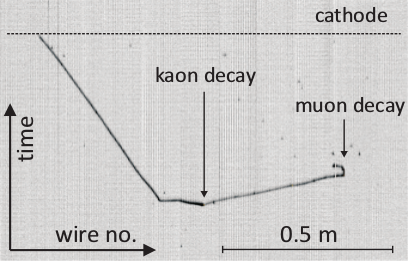
\includegraphics[width=0.8\textwidth]{fig-kaon-coll.png}
\end{dunefigure}

\begin{dunefigure}[Annotations: TikZ modified graphic]{fig:annotation-tikz}
{An image annotated using the \LaTeX Tikz package.}
\begin{tikzpicture}[scale = 1.0, font=\sffamily\LARGE]
    \node[anchor=south west,inner sep=0] at (0,0) 
    {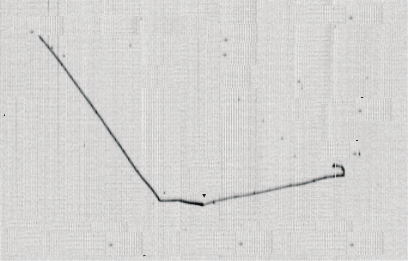
\includegraphics[width=0.8\textwidth]{fig-kaon-coll-blank.png}};
    \node at (11.7,8.5) {\textbf{cathode}};    
    \draw [line width=2pt, dotted] (0.3,7.8) -- (13.6,7.8);
    \node at (7.0,6.5) {\textbf{kaon decay}};    
    \draw [line width=1.5pt,-latex] (7.0,5.9) -- (7.0,2.1);
    \node at (11.9,5.7) {\textbf{muon decay}};    
    \draw [line width=1.5pt,-latex] (11.7,5.4) -- (11.7,3.5);
    \node at (0.9,4.1) [rotate=90] {\textbf{time}};
    \draw [line width=2pt,-latex] (0.4,0.4) -- (0.4,5.0);
    \node at (2.9,1.0) {\textbf{wire no.}};   
    \draw [line width=2pt,-latex] (0.4,0.4) -- (5.1,0.4);
    \node at (10.7,1.0) {\textbf{0.5 m}};    
    \draw [line width=1.5pt] (7.8,0.4) -- (13.5,0.4);
    \draw [line width=1.5pt] (7.8,0.2) -- (7.8,0.6);
    \draw [line width=1.5pt] (13.5,0.2) -- (13.5,0.6);    
    \draw[red,ultra thick,rounded corners] (11.3,2.5) rectangle (12.3,3.5);
\end{tikzpicture}
\end{dunefigure}


%\centerline{Figure 2.1c: \LaTeX~ TikZ Code Snippet}

\begin{dunefigure}[TikZ Code Snippet]{fig:tikz-snippet}{\LaTeX TikZ Annotation Code Snippet}
\begin{framed}
\begin{verbatim}

\begin{tikzpicture}[scale = 1.0, font=\sffamily\LARGE]
    \node[anchor=south west,inner sep=0] at (0,0) 
    {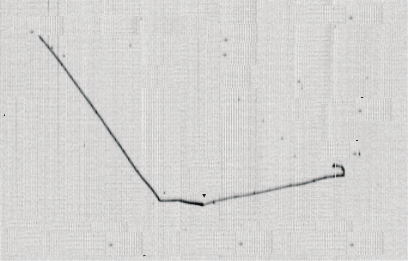
\includegraphics[width=0.8\textwidth]{fig-kaon-coll-blank.png}};
    \node at (11.7,8.5) {\textbf{cathode}};    
    \draw [line width=2pt, dotted] (0.3,7.8) -- (13.6,7.8);
    \node at (7.0,6.5) {\textbf{kaon decay}};    
    \draw [line width=1.5pt,-latex] (7.0,5.9) -- (7.0,2.1);
    \node at (11.9,5.7) {\textbf{muon decay}};    
    \draw [line width=1.5pt,-latex] (11.7,5.4) -- (11.7,3.5);
    \node at (0.9,4.1) [rotate=90] {\textbf{time}};
    \draw [line width=2pt,-latex] (0.4,0.4) -- (0.4,5.0);
    \node at (2.9,1.0) {\textbf{wire no.}};   
    \draw [line width=2pt,-latex] (0.4,0.4) -- (5.1,0.4);
    \node at (10.7,1.0) {\textbf{0.5 m}};    
    \draw [line width=1.5pt] (7.8,0.4) -- (13.5,0.4);
    \draw [line width=1.5pt] (7.8,0.2) -- (7.8,0.6);
    \draw [line width=1.5pt] (13.5,0.2) -- (13.5,0.6);    
    \draw[red,ultra thick,rounded corners] (11.3,2.5) rectangle (12.3,3.5);
\end{tikzpicture}

\end{verbatim}
\end{framed}
\end{dunefigure}

If you find the TikZ approach tedious, then at a minimum take care not to produce a 
low-quality graphic with a large filesize (>3MB). Also, please choose fonts and colors that ``work'' with the document.

If at all possible, provide the file in a format which can be further edited and which does not turn raster data into PDF nor vector data into JPEG/PNG.

If this can't be avoided and if the underlying graphic is JPEG then produce the final version in JPEG and not PNG nor PDF. If the annotation is on top of an original vector drawing and your annotation software will retain the vector information, save it as PDF.

Feel free to consult david.demuth@vcsu.edu with any assistance on creating your image annotations.



\chapter{Writing \LaTeX}

This is the start of a chapter and gives some introduction before its first section.  This chapter describes basic \LaTeX{} you need to know.

%%%%%%%%%%%%%%%%%%%%%%%%%%%%%%%%%%%%%%%%%%%%%%%%%%%%%%%%%%%%%%%%%%%%
\section{Sectioning}
\label{sec:sectioning}

The following sectioning macros are available, ordered in descending
importance:

\begin{verbatim}
\chapter{A Chapter}
\section{A Section}
\subsection{A Sub Section}
\subsubsection{A Sub Sub Section}
\subsubsubsection{A Sub Sub Sub Section}
\end{verbatim}

Three-sub's is all you get.  
Consult with the technical editors if you feel finer grained
sectioning is required.
Starting from \verb|\subsection|, this produces the following:

\subsection{A Sub Section}

This is a subsection.

\subsubsection{A Sub Sub Section}

This is a subsubsection.

\subsubsubsection{A Sub Sub Sub Section}

This is a subsubsubsection and is getting to be a bit too fine-grained. It will not appear in 
the table of contents, which will show entries as low as subsubsection only.

\subsection{Section Labels}

Just after defining a chapter and any significant section a
\verb|\label| should be added so it can be referenced.
A label can be added later for a `'less significant'' section that
turns out to need one. You can label them all. 

For example:

\begin{verbatim}
\chapter{A Chapter}
\label{ch:a-chapter}

\section{A Section}
\label{sec:a-section}

\subsection{A Sub Section}
\label{subsec:a-subsection}
\end{verbatim}

See Section~\ref{sec:refs} for how to reference labeled sections.

\FloatBarrier
%%%%%%%%%%%%%%%%%%%%%%%%%%%%%%%%%%%%%%%%%%%%%%%%%%%%%%%%%%%%%%%%%%%%
\section{Figures}
\label{sec:figures}

See Section~\ref{sec:figure-format} for guidelines on the graphics files themselves.
Instead of using the usual \texttt{figure} environment a custom \texttt{cdrfigure}
environment is used in order to provide for a consistent presentation.
The environment is called with one optional and two required
arguments:

\begin{enumerate}
\item An initial, optional short caption for the List Of Figures, in square brackets.
\item A label for referencing (it will have \texttt{fig:} prepended). Curly brackets.
\item The full caption. Curly brackets, again.
\end{enumerate}

This is followed by including the graphic file.

\begin{cdrfigure}[Short ToF caption]{aerial}{An aerial photograph of Fermilab
    showing Wilson Hall and surrounding accelerator rings (Fermilab
    Visual Media Services)}
  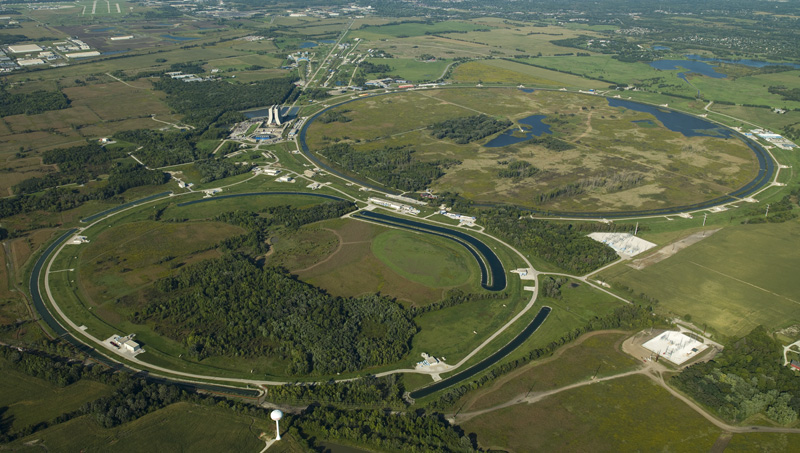
\includegraphics[width=0.8\textwidth]{fermilab-aerial.jpg}
\end{cdrfigure}


When the figure contains a graphic,  usually \texttt{includegraphics} is used.
The filename is assumed relative to a volume-specific \texttt{graphicspath} as
described in Section~\ref{sec:files} and as such one typically should
\textbf{not} specify any directory parts in its name.
The file's extension may be omitted.
An example can be seen in Figure~\ref{fig:aerial}, which is created
with the following \LaTeX shown in Figure~\ref{fig:aerial-latex}

\begin{cdrfigure}{aerial-latex}{\LaTeX{} showing how to do include a figure.}
\begin{verbatim}
\begin{cdrfigure}[Short ToF caption.]{aerial}{An aerial photograph of Fermilab
    showing Wilson Hall and surrounding accelerator rings (Fermilab
    Visual Media Services)}
  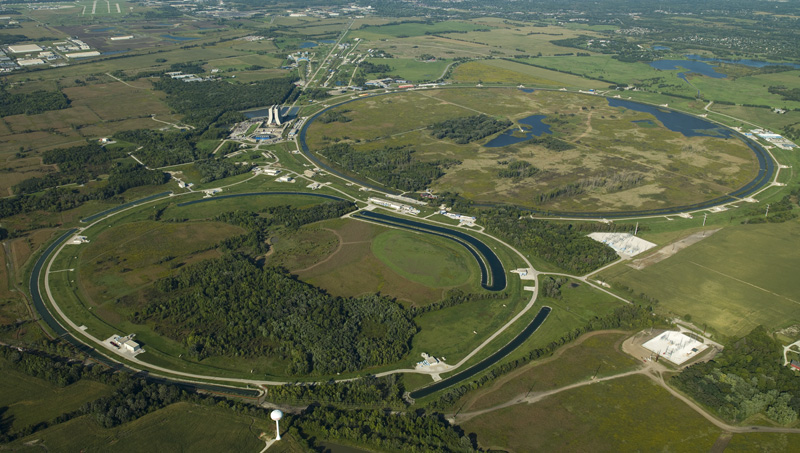
\includegraphics[width=0.8\textwidth]{fermilab-aerial.jpg}
\end{cdrfigure}
\end{verbatim}
\end{cdrfigure}

\FloatBarrier
%%%%%%%%%%%%%%%%%%%%%%%%%%%%%%%%%%%%%%%%%%%%%%%%%%%%%%%%%%%%%%%%%%%%
\section{Tables}
\label{sec:tables}

Like figures, we use a special environment, \texttt{cdrtable} for
tables to achieve a degree of consistency.
This is instead of the usual double \texttt{table} + \texttt{tabular} environments.
The \texttt{cdrtable} environment takes one optional and three
required arguments:

\begin{enumerate}
\item An initial, optional short caption for the List of Tables. Square brackets.
\item The tabular column specification. Curly brackets for the last three.
\item A label for referencing (it will have \texttt{tab:} appended)
\item The full caption.
\end{enumerate}

Inside the actual contents of the table you are required to provide a
initial row containing the headings for the table's rows followed by a
\texttt{toprowrule} macro.
Following every regular row (except the last) you should include a
\texttt{colline} macro.
Both of these take the place of the usual \texttt{hline}.

\begin{cdrtable}[The LoT caption]{cc}{example}
{This is an example table. We will use better colors, don't worry.}
  Rows & Counts \\ \toprowrule
  Row 1 & First \\ \colhline
  Row 2 & Second \\ \colhline
  Row 3 & Third \\ 
\end{cdrtable}

\noindent Table~\ref{tab:example} is thus made like (arguments can span lines):

\begin{verbatim}
\begin{cdrtable}[The LoT caption]{cc}{example}
{This is an example table. We will use better colors, don't worry.}
  Rows & Counts \\ \toprowrule
  Row 1 & First \\ \colhline
  Row 2 & Second \\ \colhline
  Row 3 & Third \\ 
\end{cdrtable}
\end{verbatim}

Table~\ref{tab:pdecay} shows a more complex example.
See the source for how it is written.
Note that special column specifications are used.

\begin{cdrtable}[Efficiencies and background rates for nucleon decay
  modes]{$L^c^c^c^c}{pdecay}{Efficiencies and background rates for
    nucleon decay channels of interest for a large underground LArTPC,
    and comparison with water Cherenkov detector capabilities} %$
  Decay Mode & \multicolumn{2}{^c}{Water Cherenkov} & 
\multicolumn{2}{^c}{Liquid Argon TPC} \\
\rowtitlestyle
& Efficiency & Background & Efficiency & Background \\ \toprowrule
$p \rightarrow K^+ \overline{\nu}$ & 19\% & 4 & 97\% & 1 \\ \colhline
$p \rightarrow K^0 \mu^+$ & 10\% & 8 & 47\% & $<2 $ \\ \colhline
$p \rightarrow K^+ \mu^- \pi^+$ & & & 97\% & 1 \\ \colhline
$n \rightarrow K^+ e^- $ & 10\% & 3 & 96\% & $<2$ \\ \colhline
$n \rightarrow e^+\pi^-$ & 19\% & 2 & 44\% & 0.8 \\
\end{cdrtable}

\FloatBarrier
%%%%%%%%%%%%%%%%%%%%%%%%%%%%%%%%%%%%%%%%%%%%%%%%%%%%%%%%%%%%%%%%%%%%
\section{Referencing and Citations}
\label{sec:refs}

Note: if you see a grey label blox containing \texttt{sec:refs}
between this paragraph and the section heading (or in general
elsewhere in chapters, sections, figures, etc), it means this document
was built in draft mode.  
These artifacts show up to help you know what label was used to
reference each particular thing.


\subsection{Intra-document References}

Assume that any chapter, section or important sub-, subsub-, section
or within any figure or table environment may need to be referenced
elsewhere in the text. As described in Section~\ref{sec:sectioning},
define a label (\verb|\label{...}| for these items.
Use the defined label in a \verb|\ref{...}| in order to make reference
to the chapter, section, figure, etc.
For example:

\begin{verbatim}
\chapter{Some Chapter}
\label{ch:some-chapter}

\subsection{Some Sub Section}
\label{subsec:some-sub-section}

...

As described in Chapter~\ref{ch:some-chapter} ...

As shown in Figure~\ref{fig:fermilab-aerial} ...
\end{verbatim}

When you reference a chapter, section, subsection, figure, table,
etc., capitalize the word ``Chapter'' or whatever it is, e.g., ``as
shown in Section~\ref{sec:plots}.''
Use the word ``Section'' even if it's a subsection or subsubsection,
and use the tilde sign to keep the number on the same line as the word
that precedes it.

Examples for figures and tables have been given above.  Here I
reference this section:~\ref{sec:refs}.  


%%%%%%%%%%%%%%%%%%%%%%%%%%%%%%%%%%%%%%%%%%%%%%%%%%%%%%%%%%%%%%%%%%%%
\subsection{Citations}

Referencing citations is done like \verb|\cite{strunk}| which gives \cite{strunk}.
(Compiling the bibliography entries into the document requires an extra step: run ``bibtex'' on
 guidance.tex, then run pdflatex on it again a couple of times. Otherwise you'll see [?] here 
 and no bibliography entry at the end.) 
The key \texttt{strunk} matches an entry in the \texttt{common/citedb.bib}
file (as relative to the top-level directory).


The \texttt{citedb.bib} file is in BibTex format.
This is \textbf{not} \LaTeX{} format and in particular does not
indicate comments via \texttt{\%} characters.
The content and order of entries in this file is not reflected in the
generated Bibliography.
However, manual care must be taken to avoid duplication.
Before adding any entry to \texttt{citedb.bib} read/search through it
to ascertain that the entry you wish to add is not already there.

\section{Common Names}

To enforce consistency, use a \LaTeX{} macro in place of any name or
term which is frequently used.
It is especially important to do this if the name or term is subject
to multiple ``spellings''.
The file \texttt{common/defs.tex} is where all such macros should be defined.

Some examples:

\begin{itemize}
\item \dm{21} is written as \verb|\dm{21}|.
\item \SURF is written as \verb|\SURF|.
\end{itemize}

\section{Numbers and Units}

\textbf{All} numerical quantities expressed as literal number
\textbf{must} have units unless they are inherently do not have a unit.
In order to enforce consistency the \texttt{siunitx} package is used
and a collection of common units are defined in
\texttt{common/units.tex}.

\subsection{Bare Numbers}

To enforce consistent writing of numbers encase them in the
\verb|\num{}| command:

\begin{itemize}
\item ``\num{100}'' is written as \verb|\num{100}|.
\item ``\num{1000}'' is written as \verb|\num{1000}|.
\item ``\num{123.456}'' is written as \verb|\num{123.456}|.
\end{itemize}

\subsection{Bare Units}

If you need to write a bare unit, one with not associated number, use
\verb|\si{}| (lower case ``si'')

\begin{itemize}
\item ``\si{m}'' is written \verb|\si{m}|.
\item ``\si{pc}'' is written \verb|\si{pc}|.
\end{itemize}

\subsection{Numbers and Units}

When a quantity has a unit write both the numerical part and the unit
using the \verb|\SI{}{}| command like:

\begin{itemize}
\item ``\SI{120}{GeV}'' is written as \verb|\SI{120}{GeV}|.
\item ``\SI{4850}{foot}'' is written as \verb|\SI{4850}{foot}|
\end{itemize}

\subsection{Adjective Quantities}

Some language uses quantities as adjectives.
These require proper outfitting with a dash which is easy to forget.
To accommodate this a set of ``adjective quantities'' commands are defined.
A generic \verb|\SIadj| is provided as are some commonly used ones.
For example:

\begin{itemize}
\item ``The \SIadj{4850}{ft} level'' is written as \verb|The \SIadj{4850}{ft} level|.
\item ``The \ftadj{4850} level'' is written as \verb|The \ftadj{4850} level|.
\item ``A typical \GeVadj{2} event'' is written as \verb|A typical \GeVadj{2} event|.
\item 
\end{itemize}

\subsection{Common compound units}

There are some common units that rather long to type out each time
especially when we require nice formatting.

\begin{itemize}
\item ``per \msr'' is written as \verb|per \msr|
\item ``exposure in \ktmwyr{}s'' is written as \verb|exposure in \ktmwyr{}s|
\end{itemize}



\chapter{English Standards for LBNF/DUNE Documents}
\label{ch:english-stds}

This chapter provides guidelines on terminology, grammar, punctuation, and other general writing guidelines for use in LBNF/DUNE documents. 


%%%%%%%%%%%%%%%%%%%%%%%%%%%%%%%%%%%%%%%%%%%%%%%%%%%%%%%%%%%%%%%%%%%%
\section{Spelling, voice, grammar and punctuation}
\label{sec:spelling}

\begin{itemize}
\item Use American spelling: e.g., ionization (not ionisation), flavor (not flavour) and so on.
\item Notice that ``e.g.,'' has two periods and a comma; so does ``i.e.,''.
\item Normally commas and periods go inside of quotations;  semi-colons and exclamation points go outside.  (In previous item, the commas are part of the terms in quotes.)
\item Use active voice as much as possible. 
\item Avoid use of first person (e.g., I and we). Use ``the team'' or ``the group,'' etc.
\item Use consistent terminology. (If you call it a spade here, call it a spade there.)
\item Expand abbreviations at first occurrence.
\item Generally, spell out numbers one through nine. Use numerals for \num{10} and above.
\item Use numerals when giving dimensions, weight, distance, etc. Other usages that always use numerals, for example, are dollars (\$1 billion, not \$\num{1000000000}), ratios, etc. Also tables often use numerals for everything.
\item For example: seven 1-ton-rated-or-less pickups ... two vans (one cargo, one equipment)... one eight-passenger suburban ...
\item Avoid starting sentences with a numeral.
\item Do not split infinitives. E.g., ``to choose carefully'' is good, but ``to carefully choose'' is bad.
\item Minimize capitalization in headings and captions.
\item Do not pluralize abbreviations using an apostrophe (') following the abbreviation. Example: CDRs are important design documents. Not CDR's. 
\begin{itemize}
\item Exception: Use an apostrophe when the abbreviation or acronym has internal periods. 
\item Exception number \num{2}: Use nu sub e plural (and others) with apostrophe; e.g., many $\nu$'s do not make light work.
\end{itemize}
\item Use of single quotation marks (') is non-standard. Best to use \emph{italics} to set off special references. Can use double quotes (``example''). 
\item Use tables and figures to highlight content. It increases readability. 
\end{itemize}



%%%%%%%%%%%%%%%%%%%%%%%%%%%%%%%%%%%%%%%%%%%%%%%%%%%%%%%%%%%%%%%%%%%%
\section{Terminology}
\label{sec:terminology}

\begin{itemize}
\item do not capitalize ``universe'' in general
\item antiwhatever not anti-whatever (e.g., antineutrino, antimatter...)
\item ``muon antineutrino,'' not ``antimuon neutrino''
\item minimum ionizing particle: MIP
\item beamline, not ``beam line'' or ``beam-line''
\item ``dual-phase,'' not ``double-phase''
\item ``detector'' should be used for the entire ND or FD, not for a module
\item use Far Detector or Near Detector with initial caps when you refer to the name of a building such as Far Detector Hall or Near Detector Hall. \item Conversly, do not capitalize ``facility'' as it is a common noun, unless the word ``facility'' is in the name of the structure.
\item ``detector module'' = any \ktadj{10} portion
\item reference FD is \SI{40}{kt}
\item for non-reference design, call it ``alternative,'' not ``alternate''
\item ``a TPC in a \ktadj{10} module,'' not ``a \ktadj{10}  TPC'' 
\item Use of ``that'' and ``which'': 
\begin{itemize}
\item Use ``that'' for restrictive clauses (clauses that cannot be removed without altering the meaning of the sentence). E.g., ``She uses the chair that goes with this desk.''
\item Use ``which'' for non-restrictive clauses (clauses that can be removed without altering the meaning of a sentence.) Tip: Use ``which'' in conjunction with a comma and check if that clause can be removed without changing the sense.  E.g., ``A desk like this, which would be too low for you, should have a chair like that.''
\end{itemize}
\end{itemize}

%%%%%%%%%%%%%%%%%%%%%%%%%%%%%%%%%%%%%%%%%%%%%%%%%%%%%%%%%%%%%%%%%%%%
\section{Abbreviations}
\label{sec:abbrevs}

\begin{itemize}
\item can use ND, FD for near and far detector
\item U.S. not US
\item Ph.D not PhD.
\item ``a'' liquid argon TPC, and also ``a'' LArTPC (i.e., a ``lar'' TPC not an ``ell-ay-are-TPC'') 
\item \si{kt} not \si{kton} (kiloton only when used as in ``a kiloton of LAr is...'') 

\end{itemize}

%%%%%%%%%%%%%%%%%%%%%%%%%%%%%%%%%%%%%%%%%%%%%%%%%%%%%%%%%%%%%%%%%%%%
\section{Hyphenation}
\label{sec:hyphen}

\begin{itemize}
\item to separate for emphasis: use two dashes together: \verb|--| in text, e.g.,  ``the system -- not to mention its three subsystems -- does such and such'' 
\item antiwhatever not anti-whatever (e.g., antineutrino, antimatter...)
\item ``muon antineutrino'' not ``antimuon neutrino''
\item beamline not ``beam line'' or ``beam-line'' 
\item world-class but worldwide   
\item readout, not read-out
\item offline, not off-line
\item co-spokespersons not co-spokespeople
\item dash in double-beta decay, (and inverse-beta decay)
\item I've been using a hyphen when first adjective modifies following adjective, not the noun. E.g. ``deep-underground location'' vs. ``located deep underground.''  This is not strictly necessary; use as you see fit.
\item ``a \ktadj{10} mass module'' (with hyphen) vs. ``module has mass of \SI{10}{kt}'' (without)
\item high-resolution detector (with hyphen) vs. high resolution of the detector (without)
\item may use ``Oxford commas'' (e.g., after the y in ``x, y, and z'')
\end{itemize}

%%%%%%%%%%%%%%%%%%%%%%%%%%%%%%%%%%%%%%%%%%%%%%%%%%%%%%%%%%%%%%%%%%%%
\section{Lists}
\label{sec:lists}

\begin{itemize}
\item In paragraphs that enumerate lists of things, use bullet or numbered lists ('itemize' or 'enumerate' in LaTeX) unless it seems overblown.
\item If bullets seem overblown,  use open-close parens with number, e.g., (1) blah, (2) blahh, ... and (n) blahhhhh. I.e., do not use other formats like 1), 2), or (a), (b)... etc.
\item Use numbers only if there is an implied order to your list; e.g., steps in a procedure, priority, etc.
\item Otherwise use bullets.
\item Use a stem sentence to introduce a list and write the stem in a complete sentence, wherever possible.
\item Avoid using the term ``list,'' ``listed,'' ``below,'' and so on, in stem sentences. It is redundant. 
\item Follow parallel construction in lists; e.g., all phrases, all single words, all sentences, all phrases beginning with an action verb, ...
\item Use the right punctuation, i.e., use periods after complete sentences. Use either commas or semicolons after phrases. No punctuation at all for lists of words. There can be variations on this.
\item Use consistent capitalization. Initial cap the first word in a list if it is a sentence or phrase. 
\item Use only up to two sub-levels of lists.
\item It is an oversight if some of the lists in this chapter don't follow all these rules!
\end{itemize}

%%%%%%%%%%%%%%%%%%%%%%%%%%%%%%%%%%%%%%%%%%%%%%%%%%%%%%%%%%%%%%%%%%%%
\section{Common errors}
\label{sec:errors}

\begin{itemize}
\item Use the term ``comprise'' to mean ``include'' not ``compose.'' The word comprise means ``to be composed of.''
\item Verbiage does not mean ``text.'' It means wasted or superfluous text.
\item Enormity does not mean huge as in ``enormous.'' Enormity means evil.
\item Do not interchange the words ``affect'' and ``effect.'' Affect is used as a verb and effect is almost always used as a noun to mean the result of a cause. (As a verb it means ``to bring about'' as in ``to effect a change.'') 
\item Use ``impact'' as a noun and not as a verb to mean ``affect.''
\item Use of ``less'' and ``fewer'': Fewer is associated with quantity that can be counted. Less is associated with volume or mass. ``Fewer people have less mass after eating at McDonald's than have more mass.''
\item Use of the word ``concur'': You concur \emph{with} someone and you concur \emph{in} an idea or an opinion. 
\item The opposite holds true with the word ``disappoint.'' You are disappointed \emph{with} something and disappointed \emph{in} someone.
\end{itemize}





\chapter{Reviewing and Editing}
\label{ch:review}


While reviewing, it is possible to mark up the document with simple
\LaTeX{} macros as provided by the ``todonotes'' class.
This class has many features but a few are more important.

Note: if you do not see the examples in this section your copy may
have been built with the ``\texttt{final}'' option turned on.

%%%%%%%%%%%%%%%%%%%%%%%%%%%%%%%%%%%%%%%%%%%%%%%%%%%%%%%%%%%%%%%%%%%%
\section{Inline Fixme}

You may prefer to place an inline note to mark up the text.
This can be accomplished with a \fixme{Think of something critical
  about this sentence} \verb|\fixme{...}| command.

%%%%%%%%%%%%%%%%%%%%%%%%%%%%%%%%%%%%%%%%%%%%%%%%%%%%%%%%%%%%%%%%%%%%
\section{Margin notes}

You can easily add notes to the \todo{run spell checker}margine  which
are associated with some text using:

\begin{verbatim}
\todo{run spell checker.}
\end{verbatim}


%%%%%%%%%%%%%%%%%%%%%%%%%%%%%%%%%%%%%%%%%%%%%%%%%%%%%%%%%%%%%%%%%%%%
\section{Highlighting}

If you wish to add a comment on some section of text you may
\hlfix{highlight it}{This shows how.}with a comment.


\begin{verbatim}
\hlfix{highlight it}{This shows how.}
\end{verbatim}




\chapter{Important Files in the Document Repository}
\label{ch:tech}

This chapter describes some of the more technical aspects of the LBNF/DUNE \LaTeX setup. Various aspects of the configuration are pulled out into separate files to keep things well organized.  Some files are meant to be edited by contributors, others are only for the technical editing team; these latter are labeled ``Please do not edit this file'' below.

%%%%%%%%%%%%%%%%%%%%%%%%%%%%%%%%%%%%%%%%%%%%%%%%%%%%%%%%%%%%%%%%%%%%
\section{The Main File}
\label{sec:tech-mainfile}

A new main file will likely be started only by the technical editors. There is one for each volume (if a document is split into volumes). It is the file that you compile to create the document or the volume. It appears in the top level directory of the repository.  These files are named \texttt{volume-(something).tex} (or \texttt{(document-name).tex} if not multi-volume). They should be the only \texttt{(name).tex} files at this directory level.

The main file...

\begin{enumerate}
\item sets the document class (see Section~\ref{sec:tech-classfile};
\item sets the graphics path;
\item inputs the preamble;
\item opens the document environment;
\item inputs the ``init'' file;
\item Redefine the volumes subtitle when document is split into volumes
\item inputs each chapter file;
\item inputs the ``final'' file (which provides the bibliographical information); and
\item closes the document environment.
\end{enumerate}

To start a new document, you would copy the \texttt{guidance.tex} to a new
name and edit as directed by the comments.  As an example, the main file of the physics volume of the DUNE TDR might be \texttt{volume-physics.tex}. 

Please do not edit this file.

%%%%%%%%%%%%%%%%%%%%%%%%%%%%%%%%%%%%%%%%%%%%%%%%%%%%%%%%%%%%%%%%%%%%
\section{The Content Files: Text and Figures}
\label{sec:tech-contentfiles}

These are the content files that you create and/or edit. Depending on the document, they may be 
collected at the top directory level of the repository or under a subdirectory. Images typically go under a \texttt{figures} directory.  

If several volumes of a document are collected into a single repository, each under its own subdirectory, it is recommended to have a \texttt{figures} directory under each subdirectory. Only figures common to multiple volumes would be placed in the top-level \texttt{figures} directory.

%%%%%%%%%%%%%%%%%%%%%%%%%%%%%%%%%%%%%%%%%%%%%%%%%%%%%%%%%%%%%%%%%%%%
\section{The \LaTeX{} Class File}
\label{sec:tech-classfile}

All of the \LaTeX{} configuration for the document that pertains to
the general LBNF/DUNE style is in the
\texttt{td-pdr.cls} file. (The name of this file may change from document to document; it will be the only \texttt{xxx.cls} file.)
The class takes some options that control high-level style, e.g.,:

\begin{verbatim}
\newcommand{\toprowrule}{
  \arrayrulecolor{gray}
  \specialrule{1.2pt}{0pt}{1pt}
  \arrayrulecolor{black}
}
\end{verbatim}

Please do not edit this file.

%%%%%%%%%%%%%%%%%%%%%%%%%%%%%%%%%%%%%%%%%%%%%%%%%%%%%%%%%%%%%%%%%%%%
\section{Document-wide \LaTeX{} Files in \texttt{common/}}
\label{sec:tech-common}

Multi-volume documents are supported and should use the
\texttt{common/} subdirectory to house any information that is to be
shared between volumes.
Because we reuse formatting from one document to the next, the single-volume documents (e.g., the ProtoDUNE-SP TDR) also use this directory.
The expected ``common'' files include:
\begin{description}
\item[\texttt{defs.tex}] macros defining common terms. You may want to work with your team to determine an appropriate set of them, then enter them into this file.
\item[\texttt{units.tex}] macros defining how to use quantities and units. You may want to add some. 
\item[\texttt{preamble.tex}] a file that largely includies the above files along with
  any extra \LaTeX{} configuration that goes before the document
  environment begins.  Please do not edit this file.
\item[\texttt{glossary.tex}] containing words and abbreviations that you want in a glossary.
\item[\texttt{citedb.bib}] the BibTeX database file (name may change; `bib' will remain the same). You will add your references here in the proper format; examples are provided at the head of the file.
\item[\texttt{init.tex}] Any content that goes in the document
  environment but before the first chapter. 
  It typically should set the title page, ToC/LoF/LoT. Please do not edit this file.
\item[\texttt{final.tex}] Any content that goes in the document after
  the last chapter. 
  It typically contains the commands related to producing the glossary and the
  bibliography.  Please do not edit this file.
  \item[\texttt{clean.sh}] When compiled in unix with pdflatex or similar, intermediate files get created. This script removes all the generated files except the output pdf.
\end{description}

The content of many of these files should in part be kept in sync
across all document repositories.

Specific documents may place additional files in this \texttt{common/}
directory that should be shared document-wide.
For example, volumes of the TDR may include a standard \texttt{common/intro.tex}.

%%%%%%%%%%%%%%%%%%%%%%%%%%%%%%%%%%%%%%%%%%%%%%%%%%%%%%%%%%%%%%%%%%%%
\section{Getting the Files and Compiling after your Changes}
\label{sec:tech-compile}

Detailed instructions for getting the files and compiling a volume are
given on main GitHub page for the repository supplying this document at
\url{https://github.com/DUNE/document-guidance}.
  


%\chapter{Sample structure for a LBNF/DUNE design document chapter}
\label{sec:design-doc}

%%%%%%%%%%%%%%%%%%%%%%%%%%%%%%%%%%%%%%%%%%%%%%%%%%%%%%%%%%%%%%%%%%%%
\section{Volume structure}

To make design documents (e.g., CDR, TDR) easier to read, it's a good idea to follow a similar structure in the presentation of each system, subsystem and component. The structure described here assumes that each major project item (e.g., far detector, near detector...) gets a dedicated volume, and each major system within the item gets a chapter.  Depending on the actual report, this may vary. (As of July 2017, it is TBD for DUNE TDR.) ``Appropriate level of detail'' may also vary.

The different volumes of the DUNE TDR will have similar introductory chapters in case someone reads that volume.  
It will always begin with the content of ``common/intro.tex'' followed by ``About this volume.''

Create an introduction section for each chapter.  For chapters about detector systems, use the APA template as a model.
The rest of this chapter illustrates the structure of the APA chapter of the single-phase detector module. It is intended to serve as a model.

%%%%%%%%%%%%%%%%%%%%%%%%%%%%%%%%%%%%%%%%%%%%%%%%%%%%%%%%%%%%%%%%%%%%
\section{Start chapter model (using APA): Introduction and scope}
\label{apa:intro-scope}

Anode Plane Assemblies (APAs) are the far detector elements utilized to sense ionization created by
charged particles traversing the liquid argon volume inside the single-phase TPC. The planes are interleaved with Cathode Plane Assemblies (CPAs), as shown in Figure..., to establish the required electric fields and form drift volumes for the charged particles. 

\fixme{Include an image of the overall system, indicating its parts. Show how the system fits into the overall detector.}

The operating principle is illustrated in Figure...

An APA consists of a rectangular framework with a fine wire mesh stretched across it, over which are wrapped four layers of sense and shielding wires...

The scope of the Anode Plane Assembly (APA) system includes the continued procurement of materials for, and the fabrication, testing, delivery and installation of the following subsystems: 

\begin{itemize}
\item stainless steel APA frame, 150 per module 
\item wire mesh that covers the frame on both sides, ...
\end{itemize}
...
%%%%%%%%%%%%%%%%%%%%%%%%%%%%%%%%%%%%%%%%%%%%%%%%%%%%%%%%%%%%%%%%%%%%
\section{Physics requirements and parameters}
\label{apa:req-param}

The full set of requirements that the APA must satisfy is documented in 
\fixme{add ref to requirements document  when it's ready, and maybe list the most important half dozen in a table here).}  

\begin{cdrtable}[Important requirements on the APA design]{p{0.8\textwidth}}{apaphysicsparams}{Important requirements on the APA design (Sample only!)}   
Requirement  \\ \toprowrule
 The APA wire spacing shall be chosen to provide high efficiency in distinguishing electron shower from photon showers \\ \colhline
 The APA wire planes shall be oriented relative to each other to optimize the measurement of high energy and low energy tracks from accelerator  \\ \colhline
 ...\\ 
\end{cdrtable}
...

\fixme{By the end of the chapter, for every requirement listed in this section, there should exist an explanation of how it will be satisfied.}

%%%%%%%%%%%%%%%%%%%%%%%%%%%%%%%%%%%%%%%%%%%%%%%%%%%%%%%%%%%%%%%%%%%%
\section{Design considerations and parameters}
\label{apa:design-consid}

%%%%%  Design to identify MIPs -- wire pitch and other params
The APA design must enable identification of minimum-ionizing particles (MIPs). This is a function of several detector parameters, including: argon purity, drift distance, diffusion, wire pitch, and Equivalent Noise Charge (ENC).  DUNE-SP requires that MIPs originating anywhere inside the active volume of the detector be reconstructed with 100$\%$ efficiency.   The choice of wire pitch, of $\sim$5\,mm, for the wire layers on the APA, combined with key parameters for other TPC systems (described in their respective sections of the TDR), is expected to enable the 100$\%$ MIP identification efficiency.

%%%%% Locate vertices, determine fiducial vol, then back to vertex...?
DUNE-SP requires that it be possible to determine the fiducial volume (via analysis) to $<$1$\%$, which in turn requires reaching a vertex resolution of $\sim$1.5\,cm along each coordinate direction. (The fiducial volume, among other factors, determines the number of target nucleons, which is a component in cross section measurements.) 
The fine granularity of the APA wires enables excellent precision in identifying the location of any vertices in an event, (e.g., the primary vertex in a neutrino interaction or gamma conversion points in a $\pi^{0}$ decay), which has a direct impact on reconstruction efficiency.
In practice, the resolution on the drift-coordinate ($x$) of a vertex or hit will be better than that on its location in the $y-z$ plane, due to the combination of drift-velocity and electronics sampling-rate...

%%%%%%%%%%%%%%%%%%%%%%%%%%%%%%%%%%%%%%%%%%%%%%%%%%%%%%%%%%%%%%%%%%%%
\section{Schedule}
\label{apa:schedule}

\fixme{How long to make and test each APA, and what is
the high level overall technically driven schedule...}


%%%%%%%%%%%%%%%%%%%%%%%%%%%%%%%%%%%%%%%%%%%%%%%%%%%%%%%%%%%%%%%%%%%%
\section{Components}
\label{sec:apa-components}



%%%%%%%%%%%%%%%%%%%%%%%%%%%%%%%%%%%%    
\subsection{APA frame}
\label{sec:apa-frame}

\fixme{Include an image of the subsystem (frame), indicating its parts. Show how the system fits into the overall system (APA).}


%%%%%%%%%%%%%%%%%% 
\subsubsection{Dimensions}
\label{sec:apa-frame-dim}

The stainless steel frame of the APA (shown in Figures ...) is 6.06\,m long, not counting electronics and mounting hardware, and 2.30\,m wide.  It is 76.2\,mm thick, made from imperial size 3-in $\times$ 4-in $\times$ 0.120-in wall rectangular tubing... 

%%%%%%%%%%%%%%%%%% 
\subsubsection{Wire loads on frame}

The many wires strung across the frame, each with a 5-N tension ($\sim$1.1 lb), apply a large, compressive, in-plane load around the perimeter of the APA...


%%%%%%%%%%%%%%%%%%%%%%%%%%%%%%%%%%%%    
\subsection{Wires}
\label{sec:apa-wires}

\fixme{Include an image of the subsystem (wires)...}

%%%%%%%%%%%%%%%%%% 
\subsubsection{Wire material}
\label{sec:apa-wires-mat}

The choices of wire material, diameter, tension and wire-placement accuracy are made to ensure proper operation of the LArTPC at voltage, and to provide the precision necessary for reconstruction...

%%%%%%%%%%%%%%%%%% 
\subsubsection{Wire tension}
\label{sec:apa-wires-tension}

The chosen tension of 5\,N, when combined with the intermediate support combs...
 
%%%%%%%%%%%%%%%%%%%%%%%%%%%%%%%%%%%%%%%%%%%%%%%%%%%%%%%%%%%%%%%%%%%%
\section{Fabrication and assembly}
\label{sec:apa-fabrication}

%%%%%%%%%%%%%%%%%%%%%%%%%%%%%%%%%%%%    
\subsection{Frame}

%%%%%%%%%%%%%%%%%% 
\subsubsection{Frame assembly}
\label{sec:apa-fabric-frame}

The APA frame is assembled with machine screws...

%%%%%%%%%%%%%%%%%% 
\subsubsection{Frame handling}
\label{sec:apa-fabric-fr-handling}

All handling of APAs in the factory is done with the long (6-m) axis of the APAs...

%%%%%%%%%%%%%%%%%%%%%%%%%%%%%%%%%%%%    
\subsection{Wiring process}
\label{sec:apa-wiring}
The wiring process uses an automated winding machine that first rotates an APA frame to the vertical landscape position...

%%%%%%%%%%%%%%%%%%%%%%%%%%%%%%%%%%%%    
\subsection{Production plan}
\fixme{Describe how many production lines, where they will be, how to handle testing and storage...}


%%%%%%%%%%%%%%%%%%%%%%%%%%%%%%%%%%%%%%%%%%%%%%%%%%%%%%%%%%%%%%%%%%%%
\section{Interfaces}
\label{sec:apa-interfaces}

\fixme{Something about the APAs interface to the cold electronics boxes, the PDS, and interconnection features will be described in the section about CR boards...}

%%%%%%%%%%%%%%%%%%%%%%%%%%%%%%%%%%%%%%%%%%%%%%%%%%%%%%%%%%%%%%%%%%%%
\section{Transport}
\label{sec:apa-transport}


%%%%%%%%%%%%%%%%%%%%%%%%%%%%%%%%%%%%%%%%%%%%%%%%%%%%%%%%%%%%%%%%%%%%
\section{QC procedures}
\label{sec:apa-qc}

Each ProtoDUNE-SP APA will be subject to a testing program during production that will demonstrate...

%%%%%%%%%%%%%%%%%%%%%%%%%%%%%%%%%%%%    
\subsection{Tension survey}
\label{sec:apa-qc-tension}

Wire tension is a critical parameter in the performance of the APA...
%%%%%%%%%%%%%%%%%%%%%%%%%%%%%%%%%%%%    
\subsection{Electrical continuity test}
\label{sec:apa-continuity}

The electrical connection of each APA wire to the cold readout electronics must be verified...
...

%%%%%%%%%%%%%%%%%%%%%%%%%%%%%%%%%%%%    
\subsection{Conclusion}
\label{sec:apa-concl}

\fixme{This section may not always be needed.}

% Leave as is: Any final content common to all volumes.
% this is added just after end of document

\cleardoublepage
\printglossaries

\cleardoublepage
%begin stuff from init per Thomas 6/2/2106
% end stuff from init
\cleardoublepage
\renewcommand{\bibname}{References}
\bibliographystyle{utphys} 
% To understand the style chosen, see:
% https://arxiv.org/hypertex/bibstyles/ (very bottom -- additions) and
% https://www.sharelatex.com/learn/Bibtex_bibliography_styles
% July 2017, AH and BV (and AM)
\bibliography{common/tdr-citedb}

\end{document}
